\begin{exercises}

\exercise 以不同的速率同时向不同方向抛出两物体。证明在运动的
时候,若不计空气阻力,它们的相对速度固定不变。

\exercise 有一水平飞行的飞机,速度为$ v _ { 0 }$,在飞机上安置一门炮,炮弹以水平速度$ v $向前射击。略去空气阻力,求

(1) 以地球为参考系时炮弹的轨迹

(2) 以飞机为参考系时炮弹的轨迹

(3) 以炮弹为参考系时飞机的轨迹

\exercise 一辆汽车尾部敞开,顶篷只盖到$A$处(图\ref{fig:02.17}),乘客可坐
\begin{wrapfigure}[7]{r}{13em}
  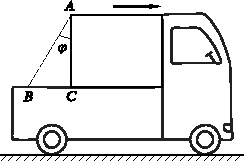
\includegraphics{figure/fig02.17}
  \caption{}
  \label{fig:02.17}
\end{wrapfigure}
到车尾$B$处,$AB$联线与铅直方向
成$ \varphi = 3 0 ^ { \circ }  $角。汽车在平直公路上
冒雨行驶,当其速率为6公里/时
时,$C$点刚好不被雨打着若它
的速率为18公里/时,则$B$点就
刚好不被雨点打着。求雨点的速
度$ v _ { 0 }$

\exercise 以速率$ v _ { 1 }  $运动的列车上的驾驶员,发现在前面与该车相距
$d$处,有一列车在同一轨道上沿相同方向、以较小的速率$v_2$在运
动,他立刻用制动器刹车,使他的火车以匀减速$a$慢下来,试证
明:

(1) 如果$d > \dfrac { \left( v _ { 1 } - v _ { 2 } \right) ^ { 2 } } { 2 a }$
则两车不会相撞;

(2) 如果$d < \dfrac { \left( v _ { 1 } - v _ { 2 } \right) ^ { 2 } } { 2 a }$
,则两车将要相撞。
% 086.jpg

\clearpage
\exercise 渔人在河中乘舟逆流航行,经过某桥下时,一只水桶落入
水中,半小时后他才发觉,即回头追赶,在桥的下游5.0公里处赶
上。设渔人顺流及逆流相对水的划行速率不变,求水流速率。

\exercise 甲乙两列火车在相邻的轨道上相向运行,甲的速率为$v_1$,
乙的速率为$v_2$。从甲车上水平地投一物到乙车上。设投掷速率为
$v _ { 0 }$ ( $v_0  $在物体运动的全部时间内可认为是不变的),从甲车上看,投
掷方向与列车行驶方向垂直,试求:

(1)物体的轨迹在路基上的投影与铁轨所成的角$ \varphi _1 $;

(2)物体的轨迹在乙车上的投影与乙车边缘所成的角$ \varphi _2 $;

(3)物体相对于路基的速度$ v' $和相对于乙车的速度$ v'' $。

\exercise 飞机罗盘指示飞机正在朝东飞行,地面情报指出,
此时刮着正南风。如果风速$ | \vec{u} | = 4 0 . 0  $公里/时,飞机相对空气的
速度为$ | \vec{v} ' | = 2 0 0  $公里/时,试用矢量图表明:飞机相对于地面的
速度$\vec{v}$;驾驶员应怎样驾驶才使其前进方向相对于地面是朝向正
东?

\exercise 一架飞机以相对于空气的匀速率$u$作水平直线飞行,从$A$飞
到$B$再返回,从$A$到$B$的距离是$L$。如果速率为$v$的风向有下列三
种情况(都有$ u > v$)  :

(1)沿着从$A$到$B$的直线

(2)垂直于从$A$到$B$的直线

(3)与$A$到$B$的直线成角。\\
试求往返一次所需要的时间。并证明,由于风的存在,往返时间
总是比无风的情况长。

\exercise 一升降机以$ a = 2 g  $的加速度从静止开始上升,在2.0秒末时
有一小钉从顶板下落,若升降机顶板到底板的距离$ k = 2 . 0  $米,求
钉子从顶板落到底板的时间$t$,它与参考系的选取有无关系?

\exercise 一飞机在海上布雷,当它在水面上高为$h$的地方以速率$v$
沿水平方向飞行时,要想使鱼雷入水时,鱼雷不与水面发生拍击,
即相对于鱼来说,水的速度完全沿鱼雷的轴线方向(图\ref{fig:02.18})。
% 087.jpg
\begin{wrapfigure}[8]{r}{15em}
  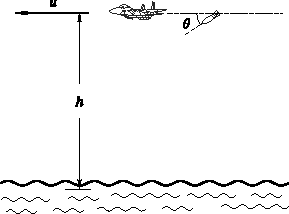
\includegraphics{figure/fig02.18}
  \caption{}
  \label{fig:02.18}
\end{wrapfigure}
设鱼雷从投下到入水,它的轴线与水平面的
夹角不变。略去空气阻力,求当飞机投射鱼雷时,$\theta$应
当等于多少?

\exercise 设某一超新星到地
球的距离$ L \geqslant 1 0 ^ { 6 }  $光年,若爆发是匀速球状膨胀,膨胀速率$|\vec{v}|$约为$5 \times 1 0 ^ { - 3 }  $光年/年。如果光速与光源速度有关,爆发后,在地球上
有多长时间间隔都能观测到它的最大光度?

\exercise 在某一参考系$K$看来,物体$A$以匀速率$v_A$沿$x$轴正向运动,
物体$B$以匀速率$v_B$沿$x$轴的负方向运动。试问:

(1) 在参考系\*$K$\*看来,\!$A$\*与\*$B$\*之间相对运动的速度\*$v_{A\!B}$\*是多大?

(2) $c$\*为真空中的光速,当\*$ v _ { A }$=0.8$ c $,\!$ v _ { B }$=\*0.6$ c  $\,时,\!$v_{A\!B}$\*是多少?

(3) 在同一参考系$K$中看来,两个物体$A$与$B$之间相对运动的
速度$ v _ { A B } > c  $,是否违反狭义相对论?为什么?

(4) 在$A$看来(即在随$A$一起运动的坐标系$K'$里看),$B$的速
度$ v _ B ' $仍旧是$v_{AB}$吗?

\exercise~ $K$和$K'$是两个相互平行的系,$K'$相对于$K$沿$x$轴以的$\dfrac { 1 } { 2 } c $速率运动。问:

(1) 在$K$系中静止放置一把尺子,长为$l$,在$K'$系来测量,尺
子的长度是多少?

(2) 在$K$系中某点$A$发生一事件,时间间隔为$\Delta t$,在$K'$系来
看,这事件的时间间隔是多少?

\exercise 在实验室中观测到一个运动着的$\mu$子在实验室坐标系中
的寿命等于静止$\mu$子寿命的50倍,求$\mu$子相对于实验室坐标系
运动
% 088.jpg
的速度$v$。

\clearpage
\exercise 爱因斯坦在他的创立狭义相对论的论文中说:“一只在
地球赤道上的钟,比放在两极的一只在性能上完全一样的钟,在
别的条件都相同的情况下,要走得慢些。”根据各种观测,地球
从形成到现在约为50亿年。假定地球形成时,就有爱因斯坦所说
的那两只钟,问:现在它们所指示的时间相差多少?已知地球半
径为6378公里。\vspace{-0.14em}

\exercise 按上题同样道理,在地球看来,一只在月球上的钟,要比
一个性质完全相同,所处条件也完全相同,放在地球上的钟走得
略为慢些。设地球年龄为$ \tau = 5 0  $亿年,月球绕地球转动的平均速率
为$ v = 1 . 0 2 \times 1 0 ^ { 5 }  $厘米/秒。月球上的钟在50亿年里比地球上的钟慢了多少?\vspace{-0.14em}

\exercise 类似15题,在太阳上的观测者将看到一只在地球上的钟,
要比一只性能完全相同、所处条件也完全相同放在太阳上的钟走
得略为慢些。设太阳年龄为$ \tau = 5 0  $亿年,已知地球公转的平均速率
为$ v = 2 9 . 7 6  $公里/秒。地球上的钟在50亿年里比太阳上的钟慢了
多少?\vspace{-0.14em}

\exercise 一个“光钟”由两个相距为$ L _ { 0 }  $的平面镜$A$和$B$组成。对于
这个光钟为静止的参考系来说,一个“滴答”的时间是光从镜面
$A$到镜面$B$再回到原处的时间,其值是$ t _ { 0 } = 2 L _ { 0 }  /c$。若将这个光钟横
放在一个以速度$\vec{v}$行驶的火车上,使两镜面都与$\vec{v}$垂直,而两镜
面中心联线则与$\vec{v}$平行。这时,若在铁轨参考系中看,火车上钟
的一个“滴答”$\tau$与$\tau _ 0$的关系怎样?\vspace{-0.14em}

\exercise ~ $\mu$子是不稳定的粒子,它自发地衰变为 \vspace{-0.2em} \\
\null\hspace{6em} $\mu ^ \pm \longrightarrow e ^ \pm + \overline{\nu} _ { e } + \nu _ { \mu }$ \vspace{-0.2em} \\
{\ziju{-0.01}其中\*$\mu ^ \pm$\*分别表示带正电或带负电的\*$\mu$\*子,\!$\overline{\nu} _ { e }$\*表示反中微子,\!$\nu _ { \mu}$\*表示$\mu$\*中微子。上述自发衰变的寿命是\*$ \tau _ { 0 }$=2.2$\times$10$^{-6}$\*秒,这是对\*$\mu$\*子静
止的坐标系而言的。\!若\*$\mu$\*子的速度\*$ v$=0.995$c$,\!它的寿命将为多少?}
\end{exercises}
